% !TEX root = ../SYSprojektrapport.tex
% SKAL STÅ I TOPPEN AF ALLE FILER FOR AT MASTER-filen KOMPILERES 

\label{Frekvensstabilitet}

Frekvensstabilitet dækker over et elektrisk systems evne til at opretholde eller hurtigt genoprette systemfrekvensen, selvom systemet påvirkes af forstyrrelse, der vil resultere i ubalance mellem produktion og belastning. Systemet skal altså kunne reguleres således at der igen opnåes balance mellem produktion og belastning i systemet, uden signifikant tab af belastning.\\
Vedvarende frekvens ustabilitet vil føre til udkobling af produktionsenheder og forbrugere.

Frekvensstabilitet inddeles i \textit{short term} og \textit{long term} stabilitetsproblemer, som vist på figur \ref{fig:Overview}.\\
\textit{Short term} har en varighed på op til 1 minut og defineres som pludselige ændringer i belastningsforholdet. Dette kunne være tab af en større generationsenhed, en transmissionslinje eller en stor forbruger. \textit{Short term} problemer kan udvikle sig til \textit{long term}, hvis systemet ikke formår med de umiddelbare tilrådige reguleringseheder ikke formår at skabe balance mellem produktion og belastning igen.\\
\textit{Long term} har en varighed fra 1 minut til flere timer og defineres som længerevarende afvigelser fra den nominelle systemfrekvens. Et \textit{long term} problem kunne opstå gennem mistiming af reguleringen af et stort synkron kraftværk grundet en forudset ændring i produktionen fra vedvarende energikilder i systemet, som følge af vejrændringer.
Typiske reguleringshastigheder er for et kulkraftværk 1\% i minuttet og for et gaskraftværk 10-15\% i minuttet.

\section{Frekvens regulering og kontrol}
Frekvensstabiliteten opretholdes i normal drift gennem handel af elektricitet, som sker på timebasis og elektricitetsmarkedet er derfor ansvarlig for at sørge produktionen matcher det forbrug markedet forventer. Ved ubalance i belastningsforholdet har Transmission System Operatoren (TSO) - i Danmark er det Energinet.dk - ansvaret for regulering af produktionen. Der defineres i ENTSO-E Policy 1\footnote{ENTSO-E Policy 1} fire forskellige kontrolreserver til at opretholde den nominelle systemfrekevens.

\begin{description}
	\item[Primær kontrol] Det enkelte kraftværks egen regulering. Kan aktiveres på sekunder.
	\item[Sekundær kontrol] Midlertidige produktionsreserve, styret af TSO'en, der kan aktiveres på sekunder/minutter med en varighed på ca 15 minutter.
	\item[Tertiær kontrol] Manuelt aktiverede produktionsreserve, styret af TSO'en. Anvendt til længerevarende ustabilitet.
	\item[Time kontrol] Handel på energimarkedet overvåges af TSO'en for at forudse behov for regulering af produktionen.
\end{description}

Måden de forskellige kontrolreserver interagerer med hinanden på kan illustres som vist på figur \ref{fig:Frekvenskontrol}. En afvigelse fra systemfrekvensen vil føre til aktivering af den primære kontrol, for at undgå tab af synkrone generationsenheder og stabilisere frekvensen ved et nyt arbejdspunkt tæt på nominel systemfrekvens. Derefter vil den sekundære kontrol aktiveres for at genoprette den nominelle systemfrekvens. Hvis den sekundære kontrol ikke formår at genoprette systemfrekvensen eller hvis generationsenheder er blevet tabt aktiveres den tertiære kontrol. Den tertiære kontrol dækker også over planlagte aktivering/regulering af produktionsenheder, der vil blive anvendt ved tab af større generationsenheder i forbindelse med forstyrrelsen/fejlen.

\begin{figure}[H] % (alternativt [H])
	\centering
	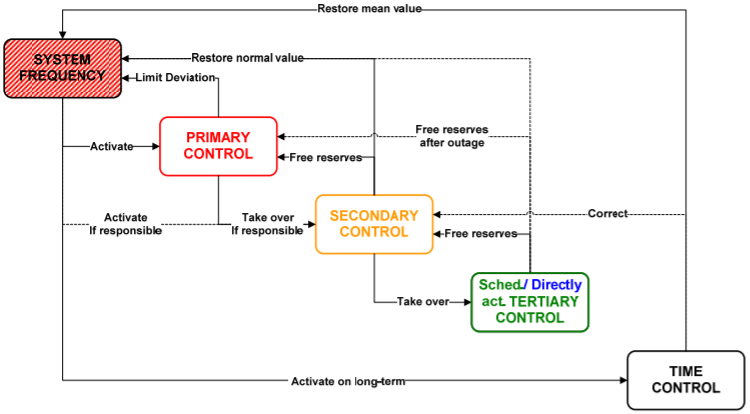
\includegraphics[width=0.9\textwidth]{figurer/Frekvenskontrol}
	\caption{Skematisk overblik over iværksættelse af kontrolreserver til frekvensregulering}
	\label{fig:Frekvenskontrol}
\end{figure}

ENTSO-E policy 1 nedsætter også nogle krav til reservekapaciteten i det centraleuropæiske elnet. Vigtige krav er at primære kontrol skal aktiveres ved frekvensafvigelser på $\pm$20mHz og den skal være fuldt ud aktiveret ved afvigelser på $\pm$200mHz. Størrelsen af den primære reserve bliver fastsat årligt og er på 3000MW.

Den primære reservekapacitet er ofte placeret ved centrale kraftværker, der er mulige at regulere....
Fortsæt her med noget relatrete til batteri implementering.



